\documentclass[10pt,a4paper]{article}

\usepackage{iftex}
\ifPDFTeX
  \usepackage[utf8]{inputenc}
  \usepackage[T1]{fontenc}
  \usepackage{lmodern}
\else
  \usepackage{fontspec} % XeLaTeX/LuaLaTeX (e.g. Tectonic): Latin Modern via fontspec
\fi
\usepackage{amsmath,amssymb,amsfonts}
\usepackage[polish]{babel}
\usepackage{graphicx}
\graphicspath{{../img/}{../assets/}{./img/}}
\usepackage{geometry}
\geometry{
    a4paper,
    margin=2.0cm
}
\usepackage{booktabs}
\usepackage{microtype}
\usepackage{xcolor}
\usepackage{xurl}
\usepackage{hyperref}
\hypersetup{
    colorlinks=true,
    linkcolor=blue!70!black,
    citecolor=blue!70!black,
    urlcolor=blue!70!black
}
\usepackage{caption}
\captionsetup{font=small, labelfont=bf, skip=6pt, justification=centering}
\usepackage{enumitem}
\setlist{itemsep=3pt, topsep=2.5pt, parsep=0.5pt}

\title{\vspace{-0.9cm}\textbf{\Large Programowanie Autonomicznych Robotów Mobilnych}\\[0.25em]
\large \textbf{Robot OmniDrive z kołami omnikierunkowymi}}
\author{}
\date{\vspace{-0.5cm}\small AGH Informatyka, 2026}

\begin{document}

\maketitle
\thispagestyle{empty}

\section{Platforma mobilna OmniDrive}

Aby robot mobilny mógł precyzyjnie nawigować w~otoczeniu, musi w~każdej chwili znać swoje położenie. Ponieważ żaden pojedynczy sensor nie zapewnia idealnego pomiaru, sterowanie platformą opiera się na fuzji danych z~wielu czujników pokładowych.

\vspace{0.15cm}
\paragraph{Wyposażenie robota OmniDrive:}
\begin{itemize}[itemsep=4.5pt, topsep=4pt, parsep=1pt]
    \item \textbf{3 koła omnikierunkowe}: rozmieszczone symetrycznie co $120^\circ$ wokół środka platformy,
    \item \textbf{Skaner laserowy 2D (LiDAR)}: optoelektroniczny dalmierz z~wirującą głowicą o~polu widzenia $240^\circ$ i~zasięgu pomiarowym do $5{,}6\text{ m}$; generuje gęstą dwuwymiarową chmurę punktów otoczenia, wykorzystywaną m.in. do budowania mapy i~lokalizacji (SLAM),
    \item \textbf{3 czujniki odległości ToF / IR (VL53L1X)}: skierowane do przodu, w~lewo i~w~prawo ($0^\circ, +90^\circ, -90^\circ$) -- optyczny pomiar odległości w~wąskim stożku wiązki laserowej,
    \item \textbf{3 czujniki ultradźwiękowe US (HC-SR04)}: skierowane do przodu, w~lewo i~w~prawo ($0^\circ, +90^\circ, -90^\circ$) -- akustyczny pomiar odległości w~szerokim stożku wiązki ultradźwiękowej,
    \item \textbf{Enkodery kół}: pomiar prędkości obrotowych oraz kąta obrotu poszczególnych kół (podstawa odometrii),
    \item \textbf{Moduł IMU / żyroskop}: bezpośredni pomiar prędkości kątowej oraz kąta orientacji $\theta$ (\emph{yaw}) platformy.
\end{itemize}

\begin{figure}[htbp]
    \centering
    \begin{minipage}[b]{0.49\textwidth}
        \centering
        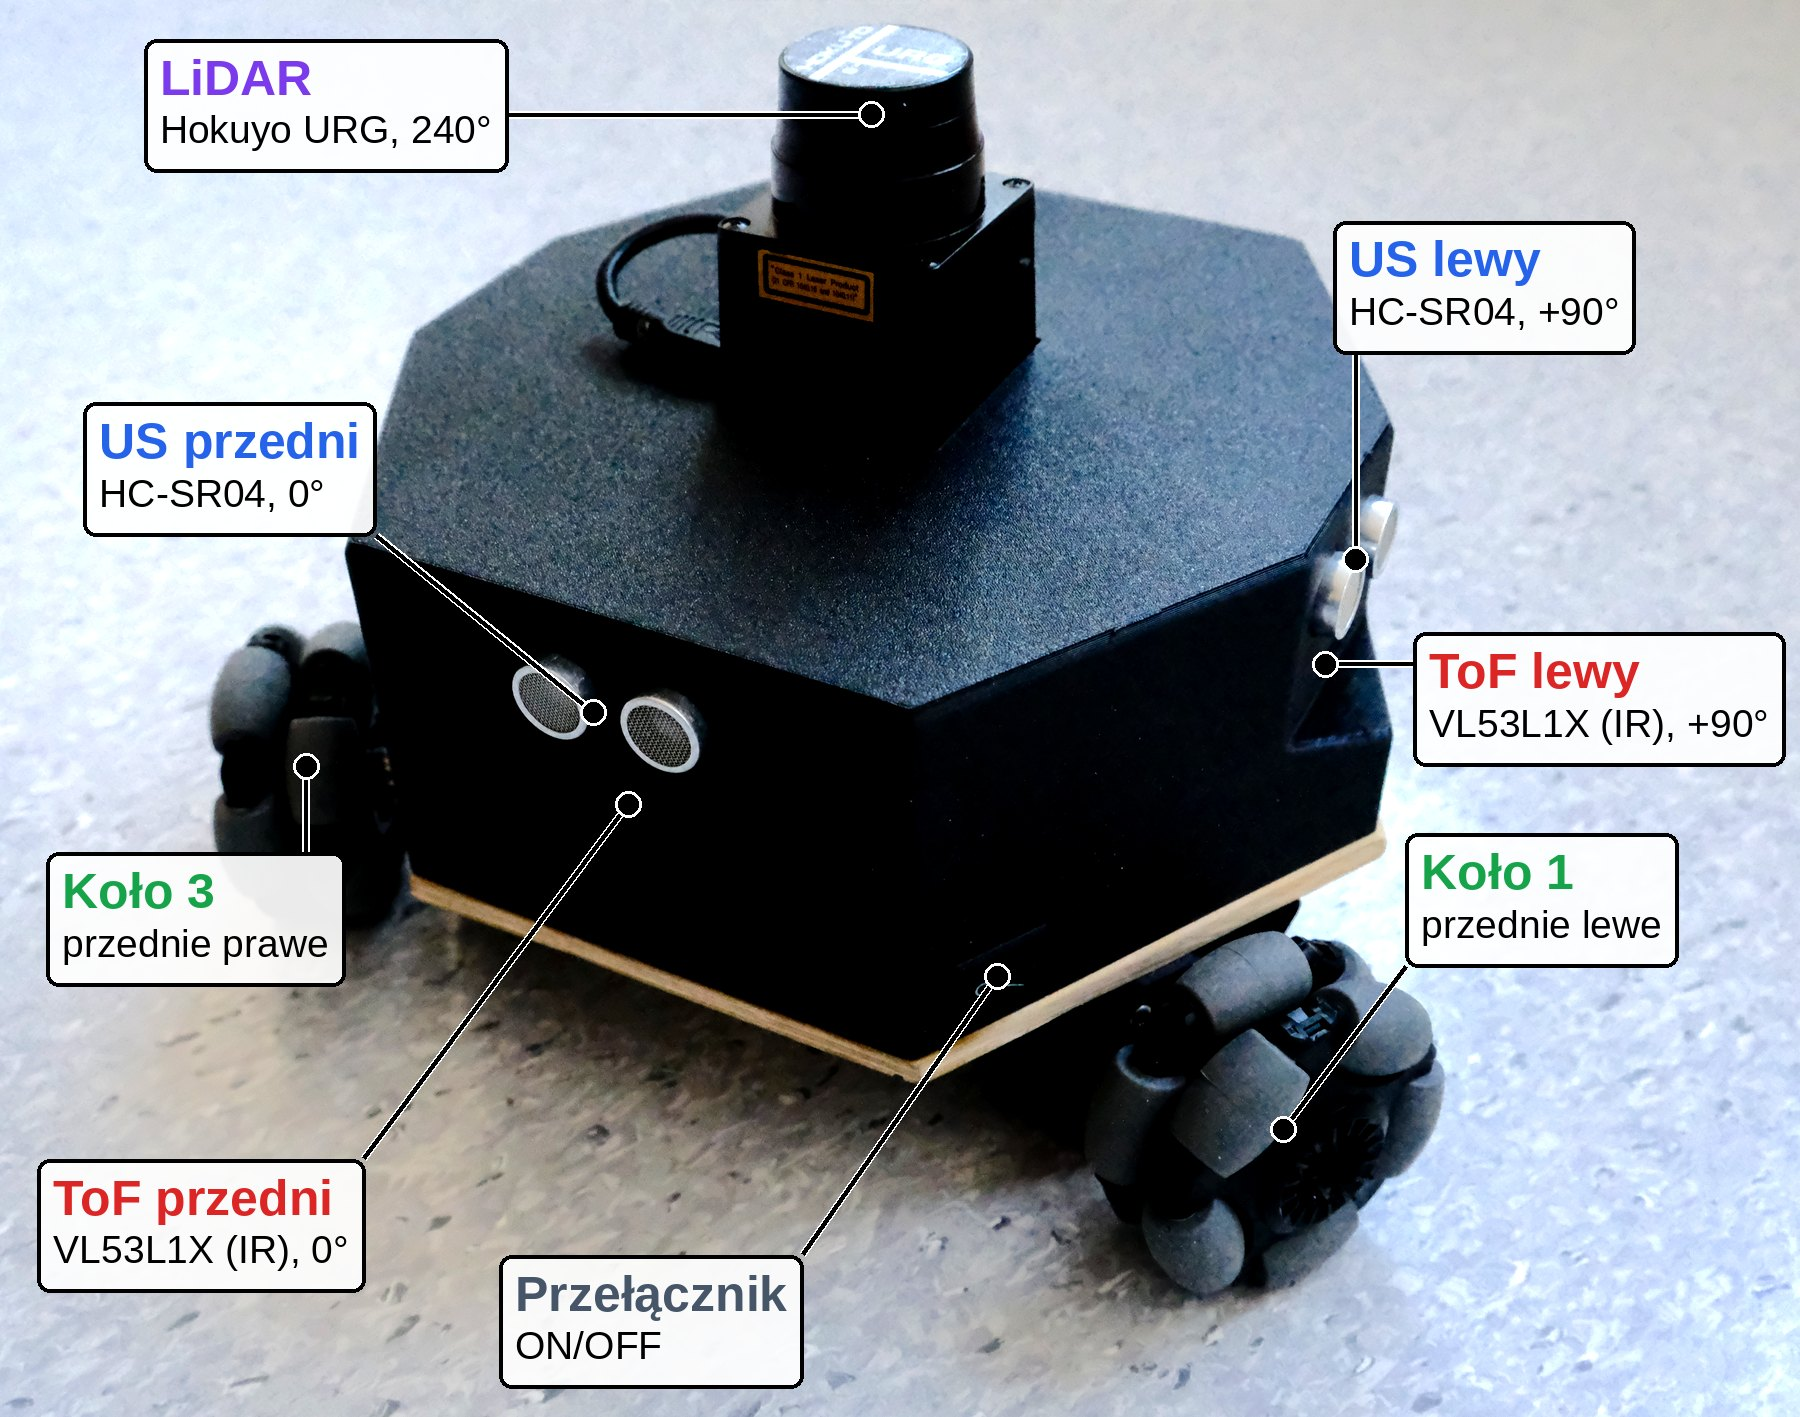
\includegraphics[width=\linewidth]{robot_front_left.jpg}\\[2pt]
        \small (a) widok z~przodu i~z~lewej
    \end{minipage}\hfill
    \begin{minipage}[b]{0.49\textwidth}
        \centering
        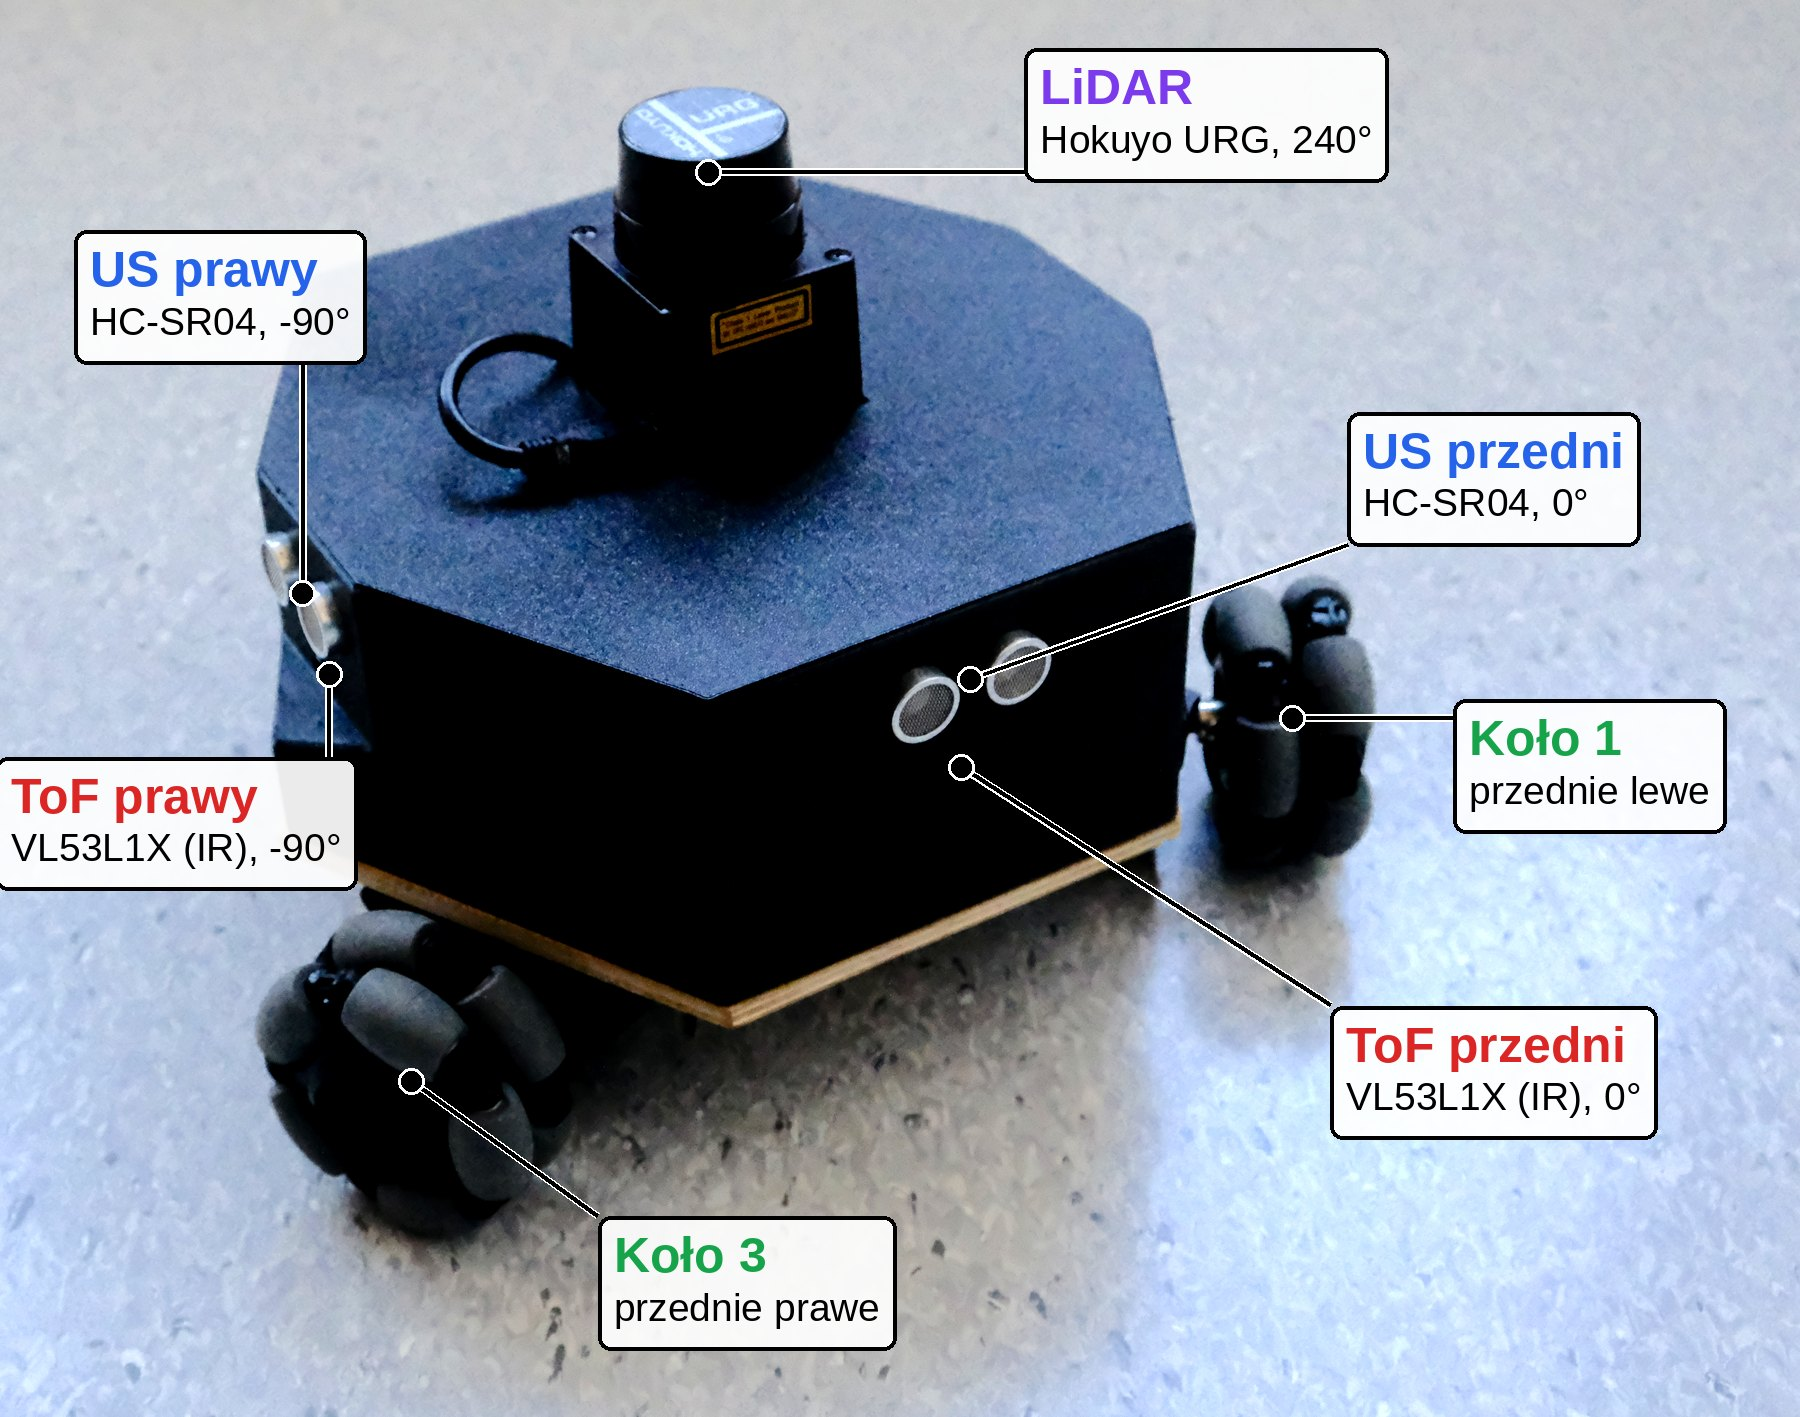
\includegraphics[width=\linewidth]{robot_front_right.jpg}\\[2pt]
        \small (b) widok z~przodu i~z~prawej
    \end{minipage}
    \caption{Robot OmniDrive: rozmieszczenie czujników, kół i~przełącznika zasilania. Kąty $0^\circ$, $+90^\circ$, $-90^\circ$ to kierunki pomiaru w~układzie robota (przód, lewo, prawo).}
    \label{fig:robot_photos}
\end{figure}

\paragraph{Rozmieszczenie elementów na robocie (rys.~\ref{fig:robot_photos} i~\ref{fig:wheel_forces}):}
\begin{itemize}[itemsep=3pt, topsep=3pt]
    \item \textbf{Obudowa}: ośmiokątny korpus drukowany w~3D, osadzony na płycie ze sklejki. \textbf{Przód} robota to płaska ściana pomiędzy kołami 1 i~3 -- to na niej znajdują się przednie czujniki US i~ToF. Koło 2 znajduje się z~tyłu.
    \item \textbf{LiDAR} (Hokuyo URG): czarny cylinder na górnej pokrywie, w~pobliżu środka robota. Wiązka laserowa obiega pole widzenia ok.~$240^\circ$ (682 pomiary na obrót) w~zasięgu $0{,}02$--$5{,}6\text{ m}$; martwa strefa znajduje się z~tyłu. Punkty bliższe niż ok.~$18\text{ cm}$ są odbiciami od samego robota i~biblioteka je pomija.
    \item \textbf{Czujniki ultradźwiękowe US} (HC-SR04): pary srebrnych cylindrów -- jeden to nadajnik, drugi odbiornik echa. Trzy zestawy: na przedniej ścianie oraz na skośnych wspornikach na lewym i~prawym boku.
    \item \textbf{Czujniki ToF / IR} (VL53L1X): niewielkie ciemne okienko tuż pod każdą parą US -- na przedniej ścianie (rys.~\ref{fig:front_sensors}) oraz na bocznych wspornikach; kryje ono nadajnik laserowy i~detektor. Każdy czujnik ToF jest skierowany tak samo jak sąsiadujący z~nim czujnik US.
    \item \textbf{Koła omnikierunkowe}: trzy koła o~promieniu $3{,}5\text{ cm}$, zamocowane $10\text{ cm}$ od środka robota. Numeracja: \textbf{koło 1} -- przednie lewe, \textbf{koło 2} -- tylne, \textbf{koło 3} -- przednie prawe.
    \item \textbf{Przełącznik kołyskowy ON/OFF}: na skośnej ścianie nad kołem 1, tuż przy płycie ze sklejki. Przycisk zasilania komputera pokładowego znajduje się pod spodem robota.
    \item \textbf{Elementy niewidoczne na zdjęciach}: enkodery silników kół (990 impulsów na obrót koła), moduł IMU, mikrokontroler ESP32 (regulacja prędkości kół i~odometria), komputer pokładowy Raspberry Pi (Wi-Fi \texttt{OmniDrive}, Jupyter) oraz akumulator ($13$--$16{,}8\text{ V}$).
\end{itemize}

\paragraph{Zasada działania kół omnikierunkowych (\emph{omni wheels}):}
Na obwodzie każdego koła znajdują się bierne rolki obracające się swobodnie w~kierunku prostopadłym do osi napędu koła. Koło przekazuje siłę na podłoże wyłącznie stycznie do okręgu platformy, a~w~kierunku poprzecznym przetacza się swobodnie bez oporu.

\vspace{0.15cm}
Dzięki trzem kołom rozmieszczonym co $120^\circ$ platforma jest \textbf{holonomiczna} -- posiada 3 niezależne stopnie swobody na płaszczyźnie $(x, y, \theta)$. Robot potrafi poruszać się w~dowolnym kierunku bez wcześniejszego skręcania i~jednocześnie obracać się wokół własnej osi.

\begin{figure}[htbp]
    \centering
    \begin{minipage}[b]{0.43\textwidth}
        \centering
        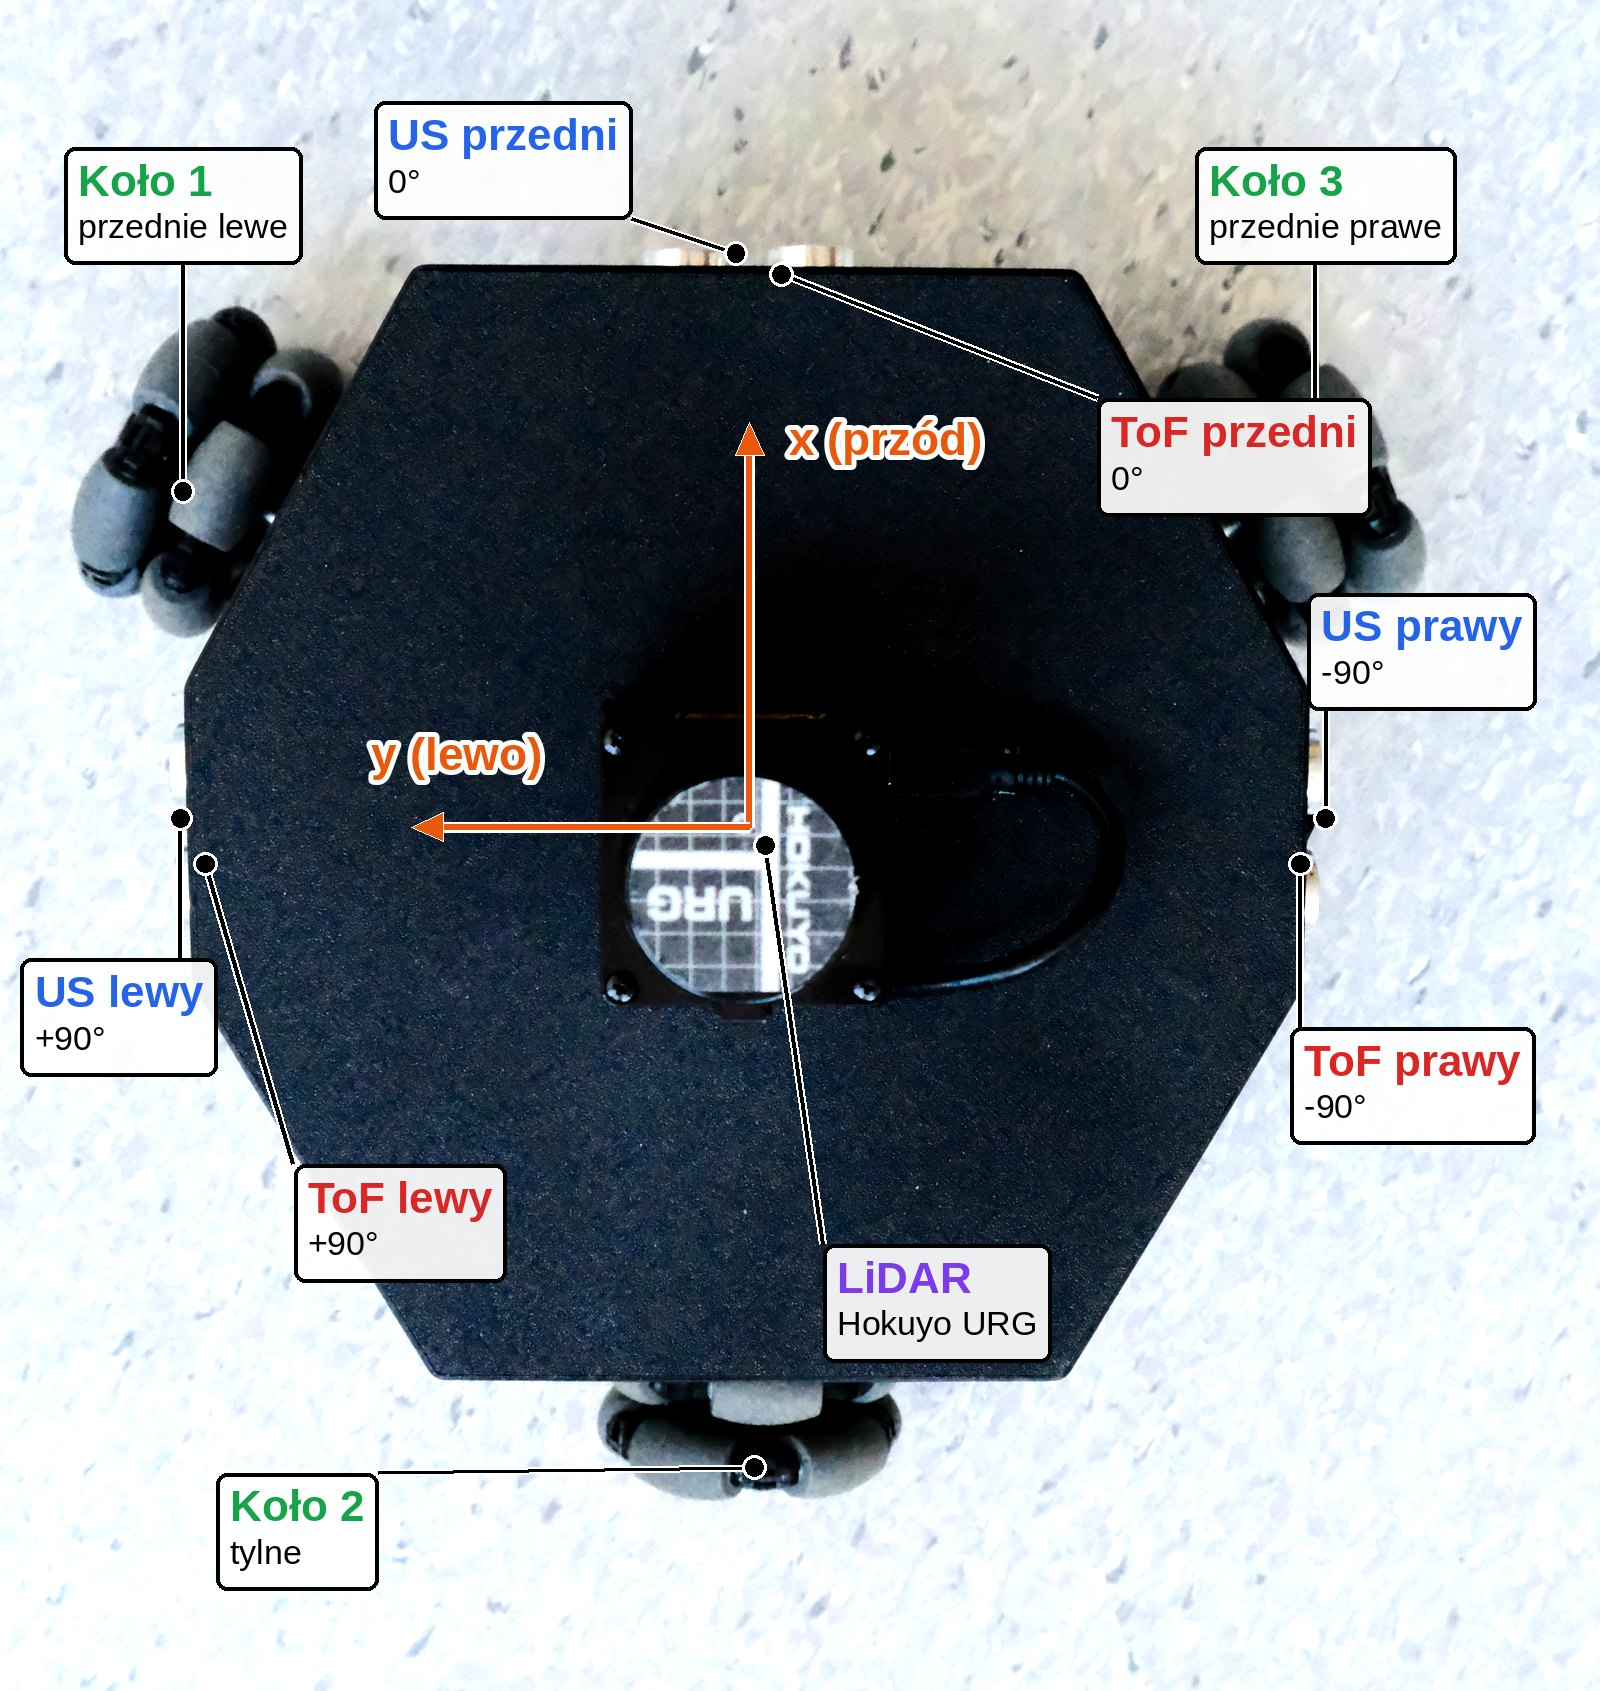
\includegraphics[width=\linewidth]{robot_top.jpg}\\[2pt]
        \small (a) robot widziany z~góry
    \end{minipage}\hspace{0.05\textwidth}
    \begin{minipage}[b]{0.43\textwidth}
        \centering
        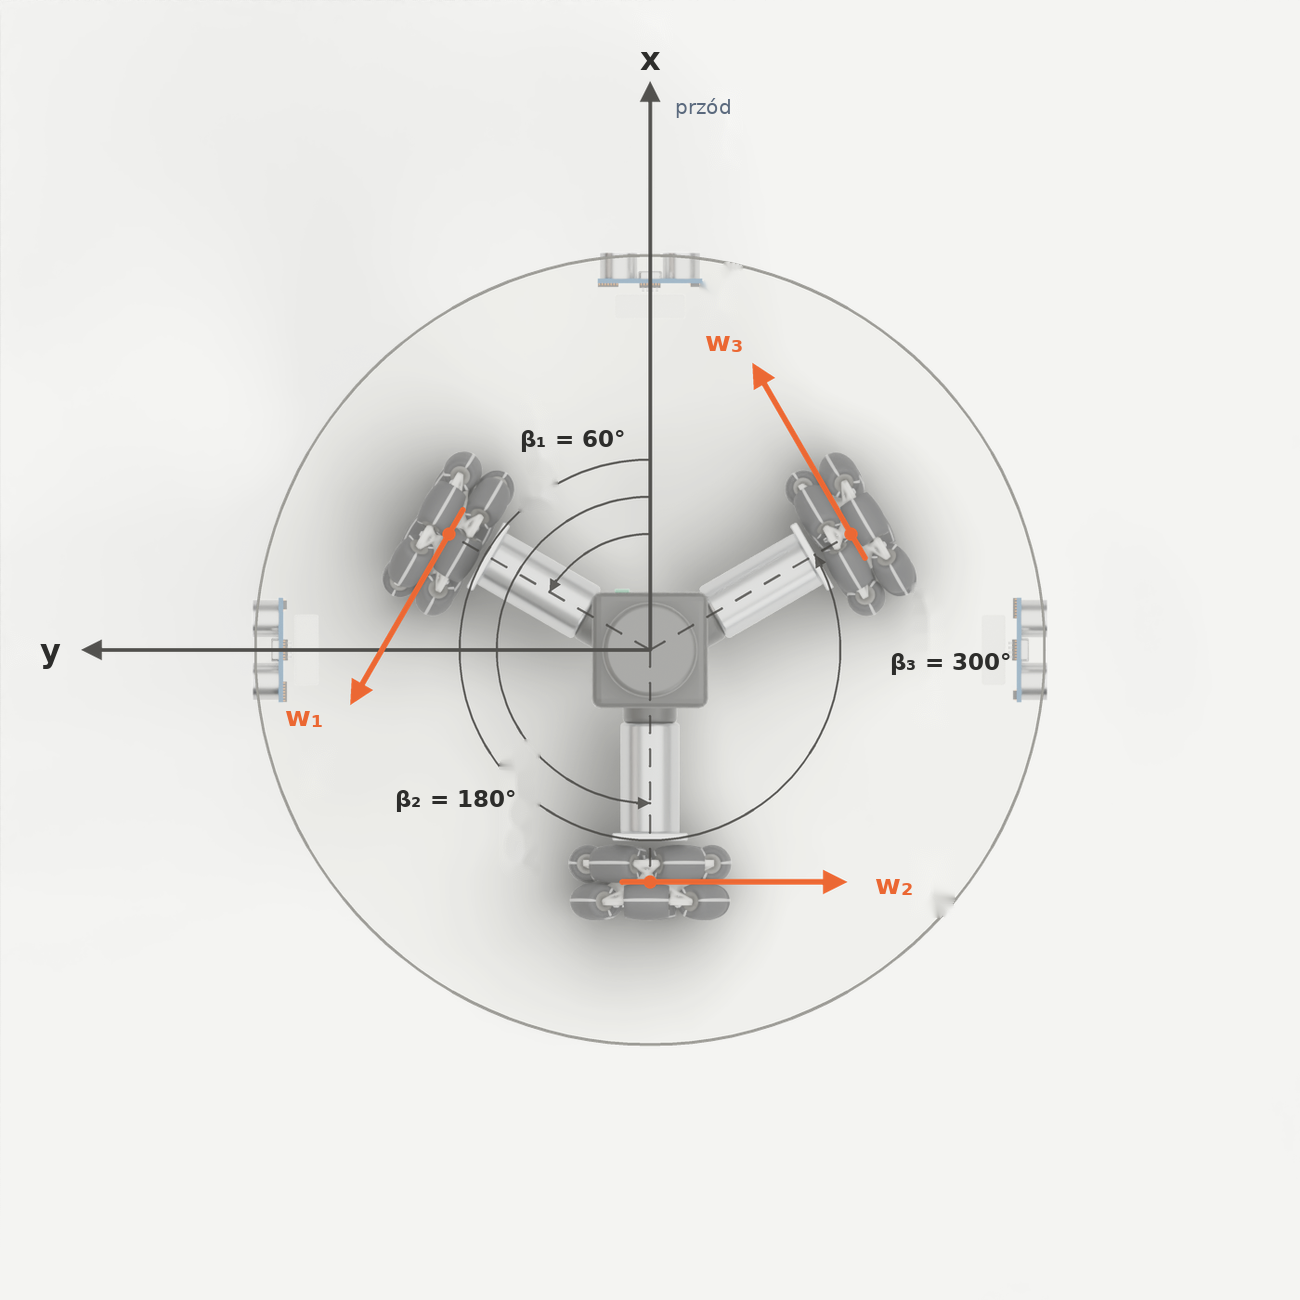
\includegraphics[width=\linewidth]{wheel_forces_top.png}\\[2pt]
        \small (b) model kinematyczny
    \end{minipage}
    \caption{Układ współrzędnych robota ($x$ -- przód, $y$ -- lewo) na rzeczywistej platformie (a) i~w~modelu ruchu (b): kąty montażowe $\beta_i$ oraz kierunki napędu kół $w_i$. Koło 1 jest przednie lewe ($\beta_1 = 60^\circ$), koło 2 tylne ($\beta_2 = 180^\circ$), koło 3 przednie prawe ($\beta_3 = 300^\circ$).}
    \label{fig:wheel_forces}
\end{figure}

\vspace{-0.1cm}
\paragraph{Kinematyka i odometria:}
\begin{itemize}[itemsep=6pt, topsep=4pt]
    \item \textbf{Kinematyka odwrotna}: odpowiada na pytanie sterowania -- jak należy napędzić poszczególne koła $(w_1, w_2, w_3)$, aby platforma poruszała się z~żądaną prędkością liniową $(v_x, v_y)$ i~kątową $\omega$.
    \item \textbf{Kinematyka prosta}: proces odwrotny, na którym bazuje \textbf{odometria}. Zlicza ona impulsy z~enkoderów kół i~przelicza ruch obwodów kół na elementarne przesunięcie robota $(\Delta x, \Delta y, \Delta\theta)$. Odometria jest szybka i~płynna, lecz działa w~pętli otwartej: mikropoślizgi i~nierówności podłoża nieuchronnie się kumulują, powodując narastający w~czasie \textbf{dryf} estymaty pozycji.
\end{itemize}

\clearpage

\section{Czujniki odległości i charakterystyka błędów pomiaru}

Do powstrzymania dryfu odometrii wykorzystujemy czujniki mierzące dystans do nieruchomych elementów otoczenia (np. ścian klatki laboratoryjnej).

\paragraph{Zasada działania sensorów:}
\begin{itemize}[itemsep=5pt, topsep=3pt]
    \item \textbf{Czujnik Time-of-Flight VL53L1X (IR)}: emituje impuls podczerwonego światła laserowego i~mierzy bezpośredni czas przelotu fotonów do przeszkody i~z~powrotem. Ma bardzo wąski stożek pomiarowy (wysoka selektywność przestrzenna), nie zależy od koloru obiektu i~działa w~zasięgu do ok.~4~m.
    \item \textbf{Czujnik ultradźwiękowy HC-SR04 (US)}: wysyła impuls akustyczny $40\text{ kHz}$ i~mierzy czas powrotu echa: $d = \frac{c \cdot t}{2}$ ($c \approx 343\text{ m/s}$). Fala rozchodzi się szerokim stożkiem. Przy przeszkodach nachylonych pod kątem występuje \textbf{odbicie zwierciadlane} -- fala odbija się w~bok i~nie wraca do sensora (brak odczytu) lub trafia rykoszetem w~inny obiekt (rys.~\ref{fig:ultrasonic}).
\end{itemize}

\begin{figure}[htbp]
    \centering
    \begin{minipage}[t]{0.42\textwidth}
        \centering
        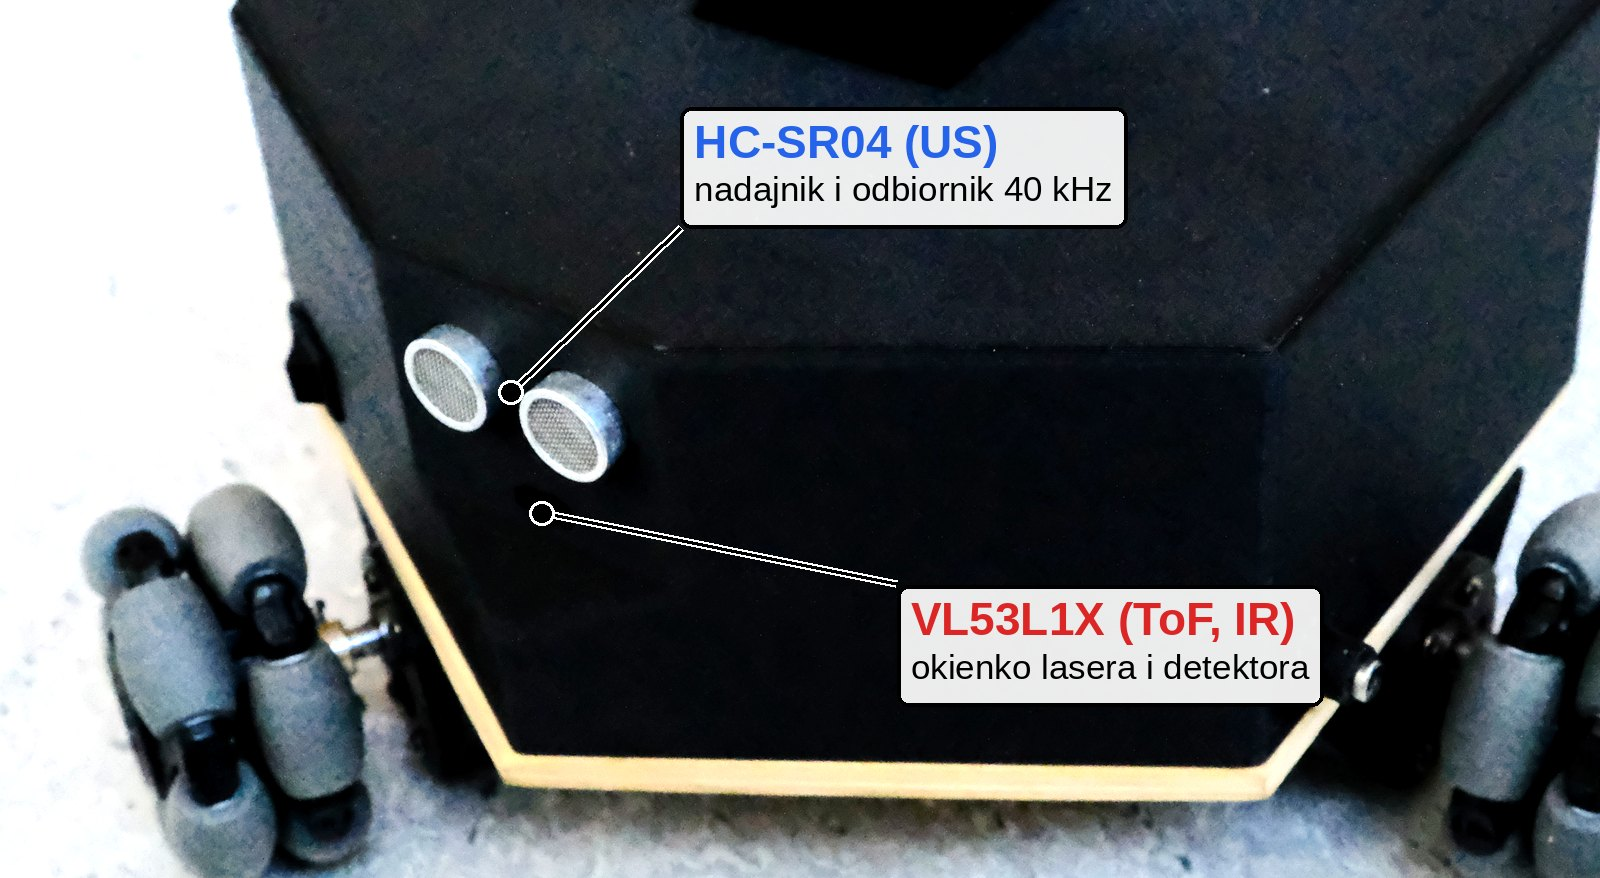
\includegraphics[width=\linewidth]{robot_front_sensors.jpg}
        \caption{Przednia ściana robota: przetworniki HC-SR04 (nadajnik i~odbiornik) oraz okienko czujnika ToF VL53L1X tuż pod nimi.}
        \label{fig:front_sensors}
    \end{minipage}\hfill
    \begin{minipage}[t]{0.54\textwidth}
        \centering
        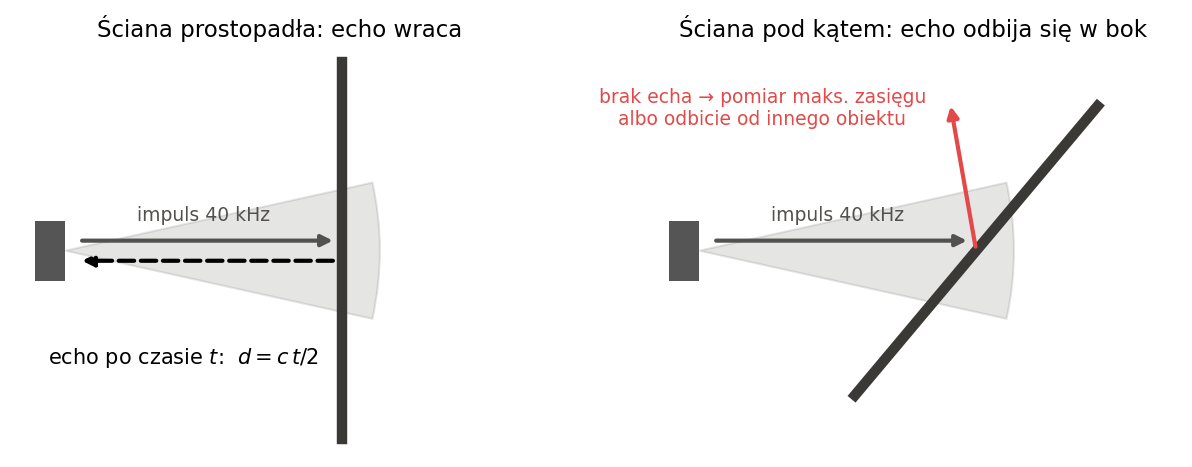
\includegraphics[width=\linewidth]{ultrasonic.png}
        \caption{Propagacja fali ultradźwiękowej: prostopadła ściana gwarantuje mocne echo; ściana ukośna powoduje odbicie fali w~bok i~utratę odczytu.}
        \label{fig:ultrasonic}
    \end{minipage}
\end{figure}

\vspace{-0.1cm}
\paragraph{Trzy rodzaje błędów pomiarowych (rys.~\ref{fig:sensor_errors}):}
\begin{enumerate}[itemsep=4pt, topsep=3pt]
    \item \textbf{Błąd systematyczny (\emph{bias})}: stałe przesunięcie wskazań względem wartości rzeczywistej (np. odległość montażowa sensora od środka robota). Usuwany przez jednorazową kalibrację (odjęcie stałego offsetu).
    \item \textbf{Szum losowy}: przypadkowe fluktuacje wokół wartości średniej, dobrze opisywane rozkładem Gaussa $\mathcal{N}(0, \sigma^2)$. Jest on skutecznie uśredniany i~tłumiony przez algorytmy filtracji.
    \item \textbf{Pomiary odstające (\emph{outliers})}: błędy grube (np. chwilowy brak echa, refleksy świetlne). Wymagają wykrycia i~odrzucenia (bramkowanie innowacji) przed fuzją danych.
\end{enumerate}

\begin{figure}[htbp]
    \centering
    \captionsetup{width=0.88\linewidth}
    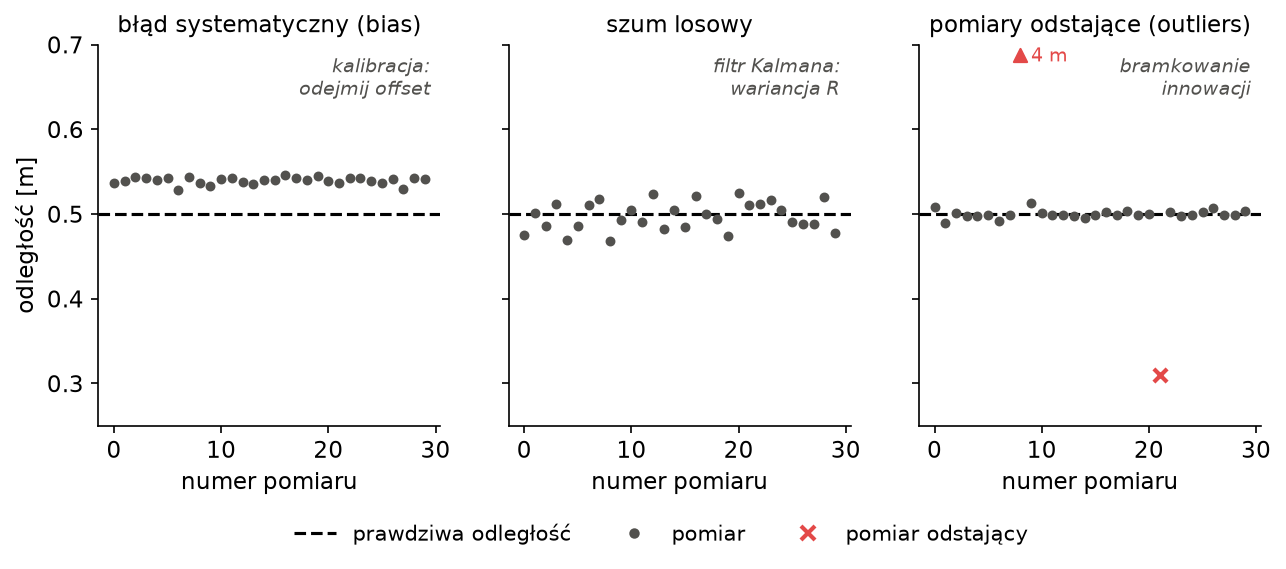
\includegraphics[width=0.76\textwidth]{sensor_errors.png}
    \caption{Charakterystyka błędów pomiarowych: błąd systematyczny (bias), szum losowy tłumiony przez filtr oraz pomiary odstające wymagające odrzucenia.}
    \label{fig:sensor_errors}
\end{figure}

\clearpage

\section{Wprowadzenie do Filtru Kalmana}

\paragraph{Dlaczego łączymy sensory?}
\begin{itemize}[itemsep=4pt, topsep=3pt]
    \item \textbf{Odometria}: jest płynna, dostępna w~każdej chwili i~reaguje natychmiast na ruch, ale ulega \textbf{nieodwracalnemu dryfowi} (błędy kumulują się bez możliwości samokorekty).
    \item \textbf{Czujniki odległości}: mierzą odległość bezwzględną do ścian (brak dryfu), ale są \textbf{zaszumione} i~podatne na zakłócenia.
\end{itemize}
Liniowy \textbf{Filtr Kalmana} łączy oba źródła, wyznaczając optymalną estymatę stanu robota $x$ (np. pozycji wzdłuż osi) wraz z~oszacowaniem jej niepewności (wariancji) $P$.

\paragraph{Pętla pracy filtru (rys.~\ref{fig:kalman_loop}):}
W~każdym kroku dyskretnym filtr wykonuje naprzemiennie dwa etapy:
\begin{enumerate}[itemsep=4pt, topsep=3pt]
    \item \textbf{Krok predykcji (\emph{ruch robota z odometrii})}:
    Przesuwamy estymatę stanu o~$\Delta x$ z~odometrii. Niepewność rośnie o~szum procesu $Q$:
    \begin{equation*}
        \bar{x} = x + \Delta x, \qquad \bar{P} = P + Q
    \end{equation*}
    \item \textbf{Krok korekty (\emph{pomiar z czujnika $z$})}:
    Pomiar $z$ reprezentuje stan obserwowany przez czujnik (dla dalmierza: odchylenie od pozycji bazowej $z = d_0 - d$). Po odebraniu pomiaru obliczamy \textbf{wzmocnienie Kalmana} $K \in [0, 1]$ oraz aktualizujemy stan i~jego wariancję ($R$ to wariancja szumu pomiaru):
    \begin{equation*}
        K = \frac{\bar{P}}{\bar{P} + R}, \qquad x = \bar{x} + K \cdot (z - \bar{x}), \qquad P = (1 - K) \cdot \bar{P}
    \end{equation*}
\end{enumerate}

\begin{figure}[htbp]
    \centering
    \captionsetup{width=0.85\linewidth}
    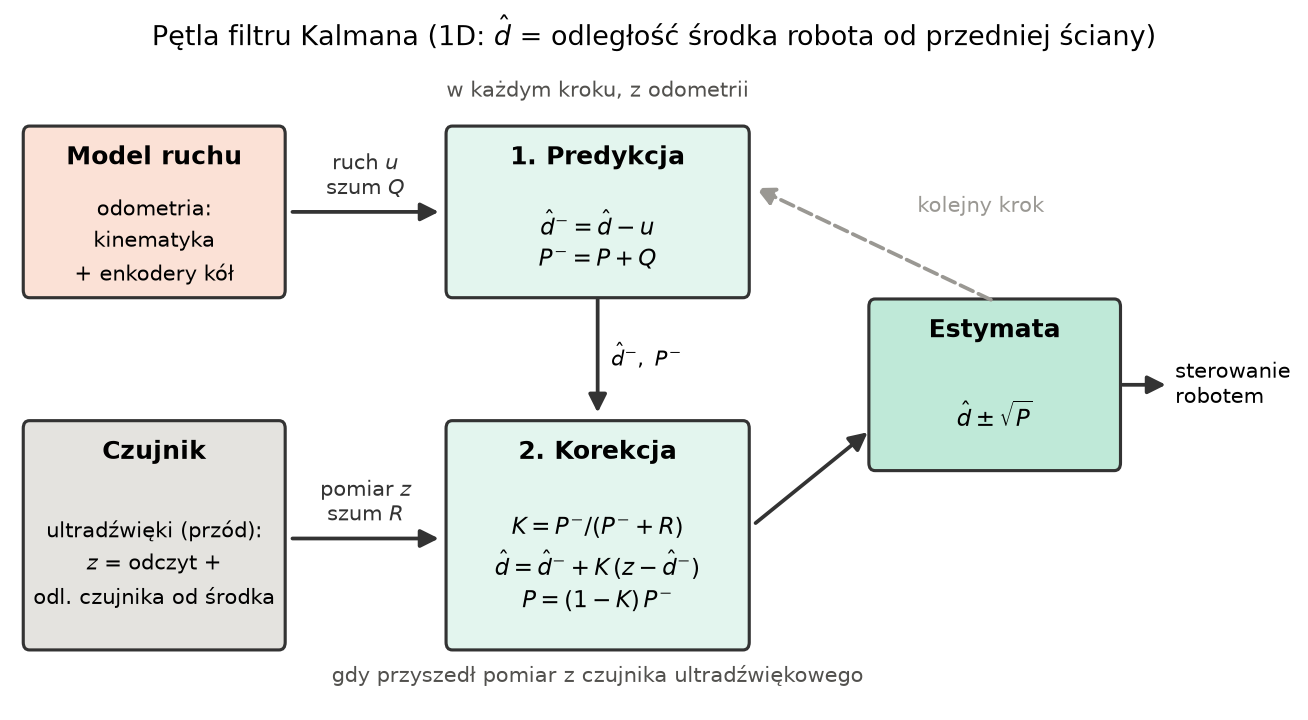
\includegraphics[width=0.52\textwidth]{kalman_loop.png}
    \caption{Pętla Filtru Kalmana w~1D: naprzemienna predykcja (na podstawie odometrii i~szumu $Q$) oraz korekta (na podstawie pomiaru z~czujnika i~szumu $R$).}
    \label{fig:kalman_loop}
\end{figure}

\paragraph{Intuicja wzmocnienia $K$ i strojenia wag $Q$ i $R$:}
\begin{itemize}[itemsep=2pt, topsep=2pt, parsep=0pt]
    \item Parametr $Q$ określa tempo wzrostu niepewności odometrii, a~$R$ to wariancja szumu pomiaru (im wyższe $R$, tym mniejsze zaufanie do pojedynczego odczytu z~czujnika).
    \item \textbf{Gdy sensor mocno szumi ($R \gg \bar{P}$)}: wówczas $K \to 0$. Filtr ignoruje pomiar i~podąża za odometrią ($x \approx \bar{x}$).
    \item \textbf{Gdy sensor jest bardzo precyzyjny ($R \ll \bar{P}$)}: wówczas $K \to 1$. Filtr natychmiast koryguje stan do pomiaru ($x \approx z$).
    \item \textbf{Redukcja niepewności}: każda poprawnie wykonana korekta zmniejsza wariancję stanu ($P < \bar{P}$).
\end{itemize}

\vspace{0.3cm}
\noindent
\setlength{\fboxsep}{7pt}%
\fcolorbox{blue!50!black}{blue!3}{%
\begin{minipage}{\dimexpr\textwidth-2\fboxsep-2\fboxrule\relax}
    \textbf{Przed zajęciami:}\par\vspace{2pt}
    Zapoznaj się z~dokumentacją \href{https://omni-drive.readthedocs.io/en/latest/}{\texttt{omni-drive.readthedocs.io}} (w~szczególności z~sekcją \emph{Getting started}). Zawiera ona dokumentację platformy OmniDrive, opis metod sterowania i~odczytu sensorów oraz przykłady użycia API.

    \vspace{4.5pt}
    \textbf{W trakcie zajęć:}\par\vspace{2pt}
    \begin{enumerate}[leftmargin=1.5em, itemsep=2.5pt, topsep=2pt, parsep=0pt]
        \item Włącz robota głównym przełącznikiem kołyskowym (\textbf{ON/OFF}) na obudowie.
        \item Pod spodem robota wciśnij przycisk zasilania -- powinien się podświetlić, a~robot zacznie się uruchamiać.
        \item Na komputerze wyszukaj sieć Wi-Fi \textbf{OmniDrive} i~połącz się z~nią (hasło: \texttt{omnidrive}).
        \item W~przeglądarce otwórz adres: \url{http://omnidrive.local} (lub alternatywnie: \url{http://10.42.0.1}).
        \item W~menu wybierz \emph{File} $\to$ \emph{New} $\to$ \emph{Terminal} i~wpisz polecenie \texttt{lab-start}. W~eksploratorze plików po lewej stronie pojawi się czysty, świeży szablon \texttt{notebook.ipynb} (jeśli plik nie jest widoczny, kliknij ikonę odświeżenia). Otwórz go i~rozpocznij wykonywanie zadań.
    \end{enumerate}

    \vspace{4.5pt}
    \textbf{Po skończonej pracy:}\par\vspace{2pt}
    \begin{enumerate}[leftmargin=1.5em, itemsep=2.5pt, topsep=2pt, parsep=0pt]
        \item W~terminalu wydaj polecenie \texttt{sudo poweroff}, aby bezpiecznie wyłączyć system.
        \item Przełącz przełącznik kołyskowy z~powrotem do pozycji \textbf{OFF}.
    \end{enumerate}
\end{minipage}%
}
\vspace{0.45cm}

\vspace{0.2cm}
\paragraph{Literatura i materiały źródłowe:}
\begin{enumerate}[label={[\arabic*]}, itemsep=1.5pt, topsep=2pt, parsep=0pt, leftmargin=1.5em]
    \small
    \item K.~Lynch, F.~Park, \emph{Modern Robotics: Mechanics, Planning, and Control}, rozdz.~13 (kinematyka robotów kołowych).
    \item G.~Welch, G.~Bishop, \emph{An Introduction to the Kalman Filter}, UNC Chapel Hill, TR~95-041.
    \item S.~Thrun, W.~Burgard, D.~Fox, \emph{Probabilistic Robotics}, MIT Press, rozdz.~3 i~7.
    \item R.~Labbe, \emph{Kalman and Bayesian Filters in Python}, \url{https://github.com/rlabbe/Kalman-and-Bayesian-Filters-in-Python}.
\end{enumerate}

\end{document}
